%-------------------------------------------------------------------------------
\FloatBarrier\section{Dynamic model of educational choice}
%-------------------------------------------------------------------------------

Please consider the standard setup of the Mincer returns as presented in class.

\begin{boenumerate}

\item Please state and briefly describe the Mincer equation \citep{Mincer.1974}. What are its key features? What important characteristics of schooling choices are lost when studying Mincer returns? What alternative return concepts exist?

\item \citet{Heckman.2006a} derive several implications of the Mincer equation and put them to the empirical test. Please provide their formal statement and a brief verbal explanation.

\end{boenumerate}\vspace{0.3cm}

Now please consider the sequential model of schooling decisions introduced in class to determine the true return to schooling.\\

Figure \ref{Decision problem} shows the two period decision problem. Individuals enter the model without any schooling and can decide to pursue up to two additional years if they desire to do so. At any point, they can drop out of school and enter the labor market with the following earnings.
%
\begin{figure}[htp]\centering
\caption{Decision problem}\label{Decision problem}
\scalebox{0.075}{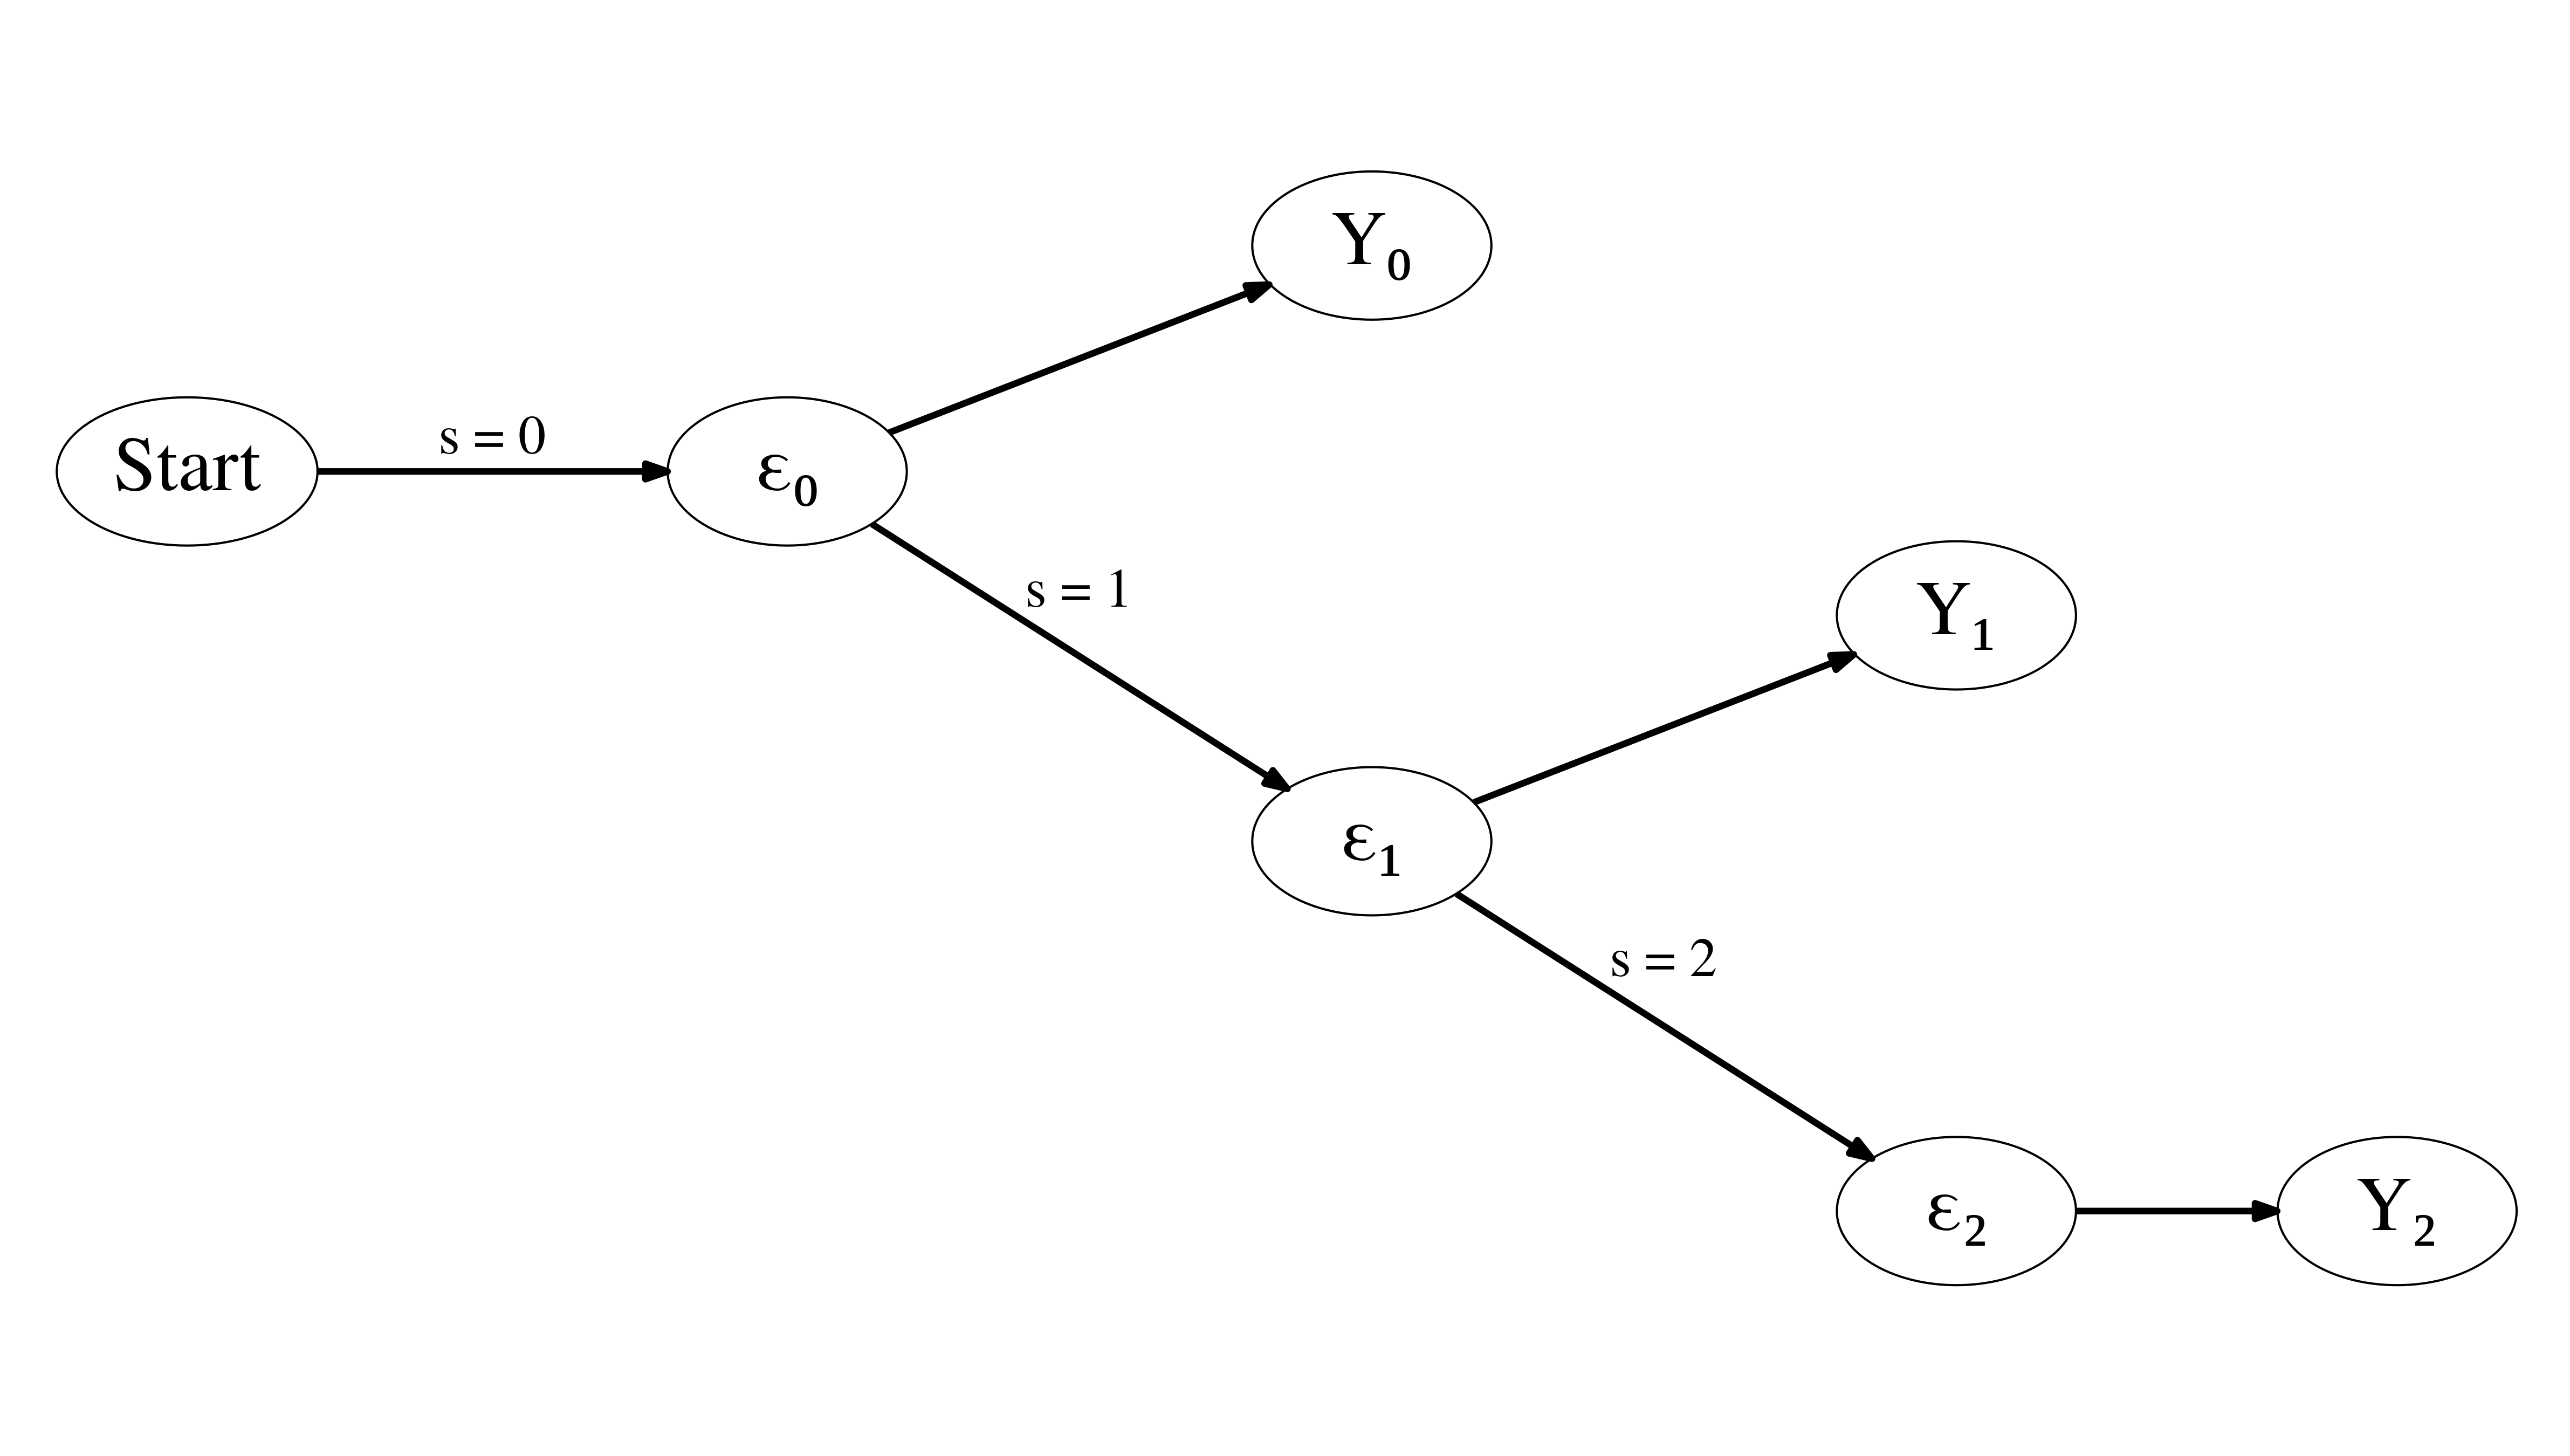
\includegraphics{fig-dynamic-model-decision-tree}}
\end{figure}
%
\begin{align*}
Y_0 = 0.5 \qquad\qquad Y_1 = 1.5 + \epsilon_1 \qquad\qquad Y_2 = 1.5
\end{align*}
%
Note that not all earnings have a random component. In addition, there is no time-discounting and $\epsilon_1$ follows a uniform distribution between zero and one.

\begin{boenumerate}\setcounter{enumi}{3}

\item What share of individuals will continue their schooling at each decision node? How does the final distribution of schooling levels look like?

\item Please provide the formal definition and a brief verbal explanation for the value  $V_s$ and true return $R_{s, s-1}$ of a schooling level. For an individual entering the model, what is the value of no schooling $V_0$ and the true return of the first year $R_{1, 0}$?

\item Please provide the formal definition and a brief verbal explanation of the option value of a schooling level. For an individual entering the model, what is the option value $O_{1, 0}$ of the first year of schooling?

\end{boenumerate}
